\documentclass[a4paper,10pt]{article}

\title{Tuto Android - Faire une aplli du feu de dieu !!}

\author{TERRIE Corentin \\ CROS Bastien \\ MONNIER Matthias}

\date{\today}

\usepackage[utf8]{inputenc}
\usepackage[french]{babel} 
\usepackage{lmodern} % Pour changer le pack de police
\usepackage{makeidx}
\usepackage{fancyhdr}
\usepackage{graphicx}
\usepackage[lofdepth,lotdepth]{subfig}
\usepackage{float}
\usepackage{hyperref}
%---------------------------------------------------------
\usepackage{listings}
\usepackage{textcomp}
% JAVA en couleur ;-)- -----------------------------------
%\lstset{
%language=Java,
%basicstyle=\normalsize, % ou ça==> basicstyle=\scriptsize,
%upquote=true,
%aboveskip={1.5\baselineskip},
%columns=fullflexible,
%showstringspaces=false,
%extendedchars=true,
%breaklines=true,
%showtabs=false,
%showspaces=false,
%showstringspaces=false,
%identifierstyle=\ttfamily,
%keywordstyle=\color[rgb]{0,0,1},
%commentstyle=\color[rgb]{0.133,0.545,0.133},
%stringstyle=\color[rgb]{0.627,0.126,0.941},
%}
%----------------------------------------------------------

\begin{document}
\makeatletter
  \begin{titlepage}
  \centering
      {\Large \textsc{École Universitaire Polytechnique de Montpellier}}\\
      \textsc{Microélectronique et Automatique - Électronique et Informatique Industrielle }\\
    \noindent\hrulefill 
    \\
    \vspace{1.5cm}
      {\large	\@date\\}
    \vspace{1.5cm}
       {\huge \textbf{\@title}} \\
	
	\vspace{0.7cm}
      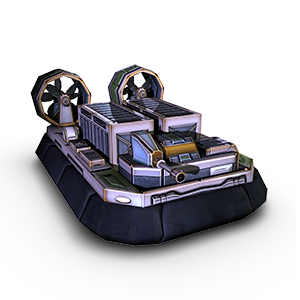
\includegraphics[scale=0.38]{head.png}\\

    \vspace{2em}
        {\large \@author} \\
    
    \vspace{2.6cm}
        
\includegraphics[height=0.15\textheight]{mea.jpg}
        \hfill
        
\includegraphics[height=0.15\textheight]{um.png}
  \end{titlepage}
\makeatother
\tableofcontents
\clearpage


%-------------------------------------------------------------------------------

\section{Notion élémentaire Watson} % Intro aux développement Android


%-------------------------------------------------------------------------------------------------------------

\section{Démarrer sous Android}
%install et tout et tout

\subsection{Sous Windows}
% Indiquer la liste des programmes

\subsection{Sous Linux}
% ligne de code nécessaire à l'install

%-------------------------------------------------------------------------------------------------------------

\section{Une première appli - Interface de base}

\subsection{App 1}
% appli basique : par exemple block note du site du zéro
\subsection{Cycle de vie d'une activité}
% 2nd partie : gestion du cycle de vie

%-------------------------------------------------------------------------------------------------------------

\section{Complexification de l'appli - Utiliser plusieurs activités}
% on améliore l'appli en affichant ce que l'on rentre dans le block note dans une seconde
% activité  

%-------------------------------------------------------------------------------------------------------------

\section{Intégration du joystick}
% on part d'une appli qui propose le choix entre joystick et gyro
% on intègre le joystic dans une nouvelle activité

%-------------------------------------------------------------------------------------------------------------

\section{Utilisation des capteurs}
% on intège les gyro dans une autre activité
Pour apprendre à utiliser les capteurs de votre support android, le tutoriel de Matthias Seguy est très bien fait. 
Voici le lien : 

\url{http://mathias-seguy.developpez.com/cours/android/android-capteurs}
%-------------------------------------------------------------------------------------------------------------

\section{Communication avec une STM}
% introduction au service
% connection BT
% programme de la stm

%-------------------------------------------------------------------------------------------------------------

\section{Foire aux conseils ;-)}
% liste des galères et leurs solutions !

\end{document}
